\documentclass[a4paper]{report}

\usepackage{graphicx}
\usepackage{float}
\usepackage{hyperref}
\usepackage{xcolor}
\usepackage[spanish]{babel}
\usepackage{listings}
\usepackage{enumitem}
\usepackage[utf8]{inputenc}
\usepackage{pdfpages}
%\usepackage{times}
%\usepackage[T1]{fontenc}
\usepackage{graphics}
%\usepackage[a4paper, top=3.5cm, bottom=2cm, left=2cm, right=2cm]{geometry}

\lstset{language=c, frame=tlrb, basicstyle=\scriptsize, breaklines=true, numberbychapter=false,numbers=left}
\setlist[enumerate]{noitemsep}
\setlist[itemize]{noitemsep}

\bibliographystyle{unsrt}

\begin{document}

\setlength{\parindent}{0cm}
\renewcommand{\tablename}{Tabla}

\title{Universidad Nacional de La Plata\\Facultad de Informática\\ \bigskip
{\large Tesis presentada para obtener el grado de \\}  Magister en Cómputo de Altas Prestaciones\\ \bigskip
  Infraestructura para el Análisis de Rendimiento}

\author{
  Alumno: Andrés More - {\tt amore@hal.famaf.unc.edu.ar}\\
  Director: Dr Fernando G. Tinetti - {\tt fernando@lidi.info.unlp.edu.ar}
}

\date{Noviembre de 2014}

\maketitle

\begin{abstract}

En el área del cómputo de altas prestaciones las aplicaciones son construidas por especialistas del dominio del problema, no siempre expertos en análisis de rendimiento y optimización.

\bigskip

Este trabajo revisa la construcción de una infraestructura que simplifica el análisis de rendimiento; incluyendo casos de estudio con aplicaciones del mundo real como etapa de validación. El objetivo es facilitar la tarea evitando la recolección de datos relevantes de modo manual, permitiendo más tiempo de experimentación y análisis.

\bigskip

En particular, este trabajo contribuye con un generador automático de reporte de rendimiento para aplicaciones de cómputo de altas prestaciones utilizando tecnología {\it OpenMP} sobre sistemas {\it GNU/Linux}.

\end{abstract}

\tableofcontents

\chapter{Introducción}

Este capítulo introduce el tema bajo estudio, definiendo los objetivos principales, las contribuciones logradas durante la investigación, y detallando la estructura del resto del documento.

\section{Motivación}

En el área de cómputo de altas prestaciones los desarrolladores son los mismos
especialistas del dominio del problema a resolver. Las rutinas
más demandantes de cálculo son en su mayoría científicas y su
alta complejidad hace posible su correcta implementación sólo por los mismos investigadores.
Estas cuestiones resultan en un tiempo reducido de análisis de resultados
e impactan directamente en la productividad de los grupos de investigación y
desarrollo.

\bigskip

Con mayor impacto que en otras áreas de la computación, el código
optimizado correctamente puede ejecutarse órdenes de magnitud mejor que una implementación
directa \cite{mm-tool}. Además, se utiliza
programación en paralelo para obtener una mejor utilización de la
capacidad de cómputo disponible; aumentando por lo tanto la complejidad de
implementación, depuración y optimización \cite{is-parallel-programming-hard}.

\bigskip

Frecuentemente el proceso de optimización termina siendo
hecho de modo {\it ad-hoc}, sin conocimiento pleno de las herramientas disponibles y
sus capacidades, y sin la utilización de información cuantitativa para dirigir los
esfuerzos de optimización. Es incluso frecuente la implementación directa
de algoritmos en lugar de la utilización de librerías ya disponibles, optimizadas
profundamente y con correctitud comprobada.

\section{Objetivos}

La propuesta principal consiste en el desarrollo de una infraestructura de soporte para el análisis de aplicaciones de cómputo de altas prestaciones ({\it HPC}, por sus siglas en inglés). Este trabajo se realiza como extensión al trabajo final {\it Herramientas para el Soporte de Análisis de Rendimiento} de la Especialización en Cómputo de Altas Prestaciones y Tecnología Grid.

\bigskip

La infraestructura desarrollada implementa un procedimiento de análisis de rendimiento ejecutando pruebas de referencia, herramientas de perfil de rendimiento y análisis de resultados. La infraestructura genera como etapa final un informe detallado que soporta la tarea de optimización con información cuantitativa.
El reporte final incluye datos estadísticos de la aplicación y el sistema donde se ejecuta, además de gráficos de desviación de resultados, escalamiento de problema y cómputo e identificación de cuellos de botella.

\section{Contribuciones}

La siguiente lista enumera las diferentes publicaciones realizadas durante el cursado del magister y el desarrollo de la tesis.

\begin{enumerate}
\item Estudio de Multiplicación de Matrices. Reporte Técnico. Realizado como parte del curso {\it Fundamentos de Procesamiento Paralelo} dictado por el Dr {\it Fernando Tinetti Laiouf}.
\item Articulo {\it Optimizing Latency in Beowulf Clusters}. HPC Latam 2012.
\item Comparación de Implementaciones de una Operación BLAS. Reporte Técnico. Realizado como parte del curso {\it Programación GPU de Propósito General} dictado por la Dra {\it Margarita Amor}.
\item Sección {\it Intel Cluster Ready} y {\it Intel Cluster Checker} en el libro {\it Programming Intel Xeon Phi}. Intel Press. 2013.
\item Reseña del Libro {\it Intel Xeon Phi Coprocessor High Performance Programming} - JCS\&T Vol 13 N 2 Octubre 2013.
\item Articulo {\it Lessons learned from contrasting BLAS kernel implementations} - XIII Workshop Procesamiento Distribuido y Paralelo (WPDP), 2013.
\end{enumerate}

\section{Metodología}

En base al problema y a los objetivos establecidos previamente, la metodología adoptada es la siguiente:

\begin{enumerate}
\item Dado el procedimiento propuesto anteriormente, automatizarlo y analizar potenciales mejoras hacia generalidad y utilidad.
\item Identificar que tipos de gráficos y tablas pueden resumir la información obtenida y facilitar su utilización.
\item Utilizar la infraestructura generando reportes de núcleos de cómputo conocidos para poder focalizar los esfuerzos en la mejora del reporte.
\item Por último, probar con aplicaciones del mundo real y verificar que la información reunida es útil para el análisis del rendimiento.
\end{enumerate}

\section{Estructura}

El resto del documento se estructura de la siguiente forma:

\begin{itemize}
\item Capitulo 2: revisa el estado del arte de los temas incluidos.
\item Capitulo 3: describe el problema a resolver.
\item Capitulo 4: muestra la propuesta de solución.
\item Capitulo 5: aplica la solución a casos de estudio.
\item Capítulo 6: concluye reflejando los objetivos y proponiendo trabajo futuro.
\end{itemize}

\chapter{Estado del Arte}

Este capítulo revisa el estado del arte de los temas relevantes a esta tesis.

\section{Análisis de Rendimiento}\label{chapter:analysis}

Este capítulo introduce el concepto de rendimiento y teoría básica sobre su análisis.
Además ejemplifica las actividades a realizar durante el análisis.

\subsection{Definición}

El rendimiento se caracteriza por la cantidad de trabajo de cómputo que se
logra en comparación con la cantidad de tiempo y los recursos ocupados.
El rendimiento debe ser evaluado entonces de forma cuantificable, utilizando alguna
métrica en particular de modo de poder comparar relativamente dos sistemas o
el comportamiento de un mismo sistema bajo una configuración distinta.

\subsection{Paralelismo}

Una vez obtenida una implementación eficiente, la única alternativa para mejorar el rendimiento es explotar el paralelismo que
ofrecen los sistemas de cómputo. Este paralelismo se puede explotar a diferentes niveles, desde instrucciones especiales que ejecutan sobre varios
datos a la vez (vectorización), hasta la utilización de múltiples sistemas para distribuir el trabajo.

\bigskip

 El cálculo de las mejoras posibles de rendimiento, cómo priorizarlas y la estimación de su límite máximo es una tarea compleja. Para ello existen algunas leyes fundamentales utilizadas durante el análisis de rendimiento.

\subsubsection{Ley de {\it Amdahl}}

 La ley de {\it Amdahl} \cite{amdahl} dimensiona la mejora que puede obtenerse en un sistema de acuerdo a las mejoras logradas en sus componentes. Nos ayuda a establecer un límite máximo de mejora y a estimar cuales pueden ser los resultados de una optimización.

\bigskip

La mejora de un programa utilizando cómputo paralelo está limitado por el tiempo necesario para completar su fracción serial o secuencial. En la mayoría de los casos, el paralelismo sólo impacta notoriamente cuando es utilizado en un pequeño número de procesadores, o cuando se aplica a problemas altamente escalables ({\it Embarrassingly Parallel Problems}). Una vez paralelizado un programa, los esfuerzos suelen ser enfocados en cómo minimizar la parte secuencial, algunas veces haciendo más trabajo redundante pero en forma paralela.

\bigskip

Suponiendo que una aplicación requiere de un trabajo serial más un trabajo paralelizable, la ley de {\it Amdahl} calcula la ganancia ($ S $) mediante la Ecuación \ref{eq:amdahl}.
Donde $ P $ es el porcentaje de trabajo hecho en paralelo, ($ 1-P $) es entonces el trabajo en serie o secuencial, y $ N $ la cantidad de unidades de cómputo a utilizar.

\begin{eqnarray}
\label{eq:amdahl}
S = \frac{1}{(1 - P) + \frac{P}{N}}
\end{eqnarray}

Esta ley nos establece que incluso teniendo infinitas unidades de cómputo la ganancia está limitada.
La Tabla \ref{fig:amdahl} muestra que no importa la cantidad de unidades de
procesamiento que sean utilizadas.

\begin{table}[H]
\caption{Mejora Máxima}
\centering
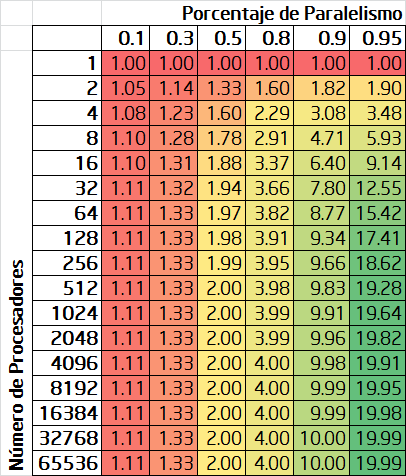
\includegraphics[width=7cm]{amdahl.png}

\label{fig:amdahl}
\end{table}

Por ejemplo, en el caso de tener solo un $ 10\% $ de paralelismo
en una aplicación, la mejora nunca va a superar $ 1.10x $ la original.
En el caso de tener un $ 95\% $, la mejora no puede ser mayor a $ 20x $.

\bigskip

En el caso de conocer los tiempos de ejecución para distinto número de procesadores, la porción serial/paralelo puede ser aproximada mediante la siguiente ecuación:

\begin{equation}
P = TBD1
S = TBD2
\end{equation}

\subsubsection{Ley de {\it Gustafson}}

Desde un punto de vista más general, la ley de {\it Gustafson}
\cite{gustafson} (Ecuación \ref{eq:gustafson})
establece que las aplicaciones que manejan problemas
repetitivos con conjuntos de datos similares pueden ser fácilmente
paralelizadas. En comparación, la ley anterior no escala el tamaño o
resolución de problema cuando se incrementa la potencia de cálculo, es
decir asume un tamaño de problema fijo. 

\begin{eqnarray}
\label{eq:gustafson}
speedup(P) = P - \alpha \times ( P - 1)
\end{eqnarray}

donde $ P $ es el número de unidades de cómputo y $ \alpha $ el porcentaje de trabajo paralelizable.

\bigskip

Al aplicar esta ley obtenemos que un problema con datos grandes o repetitivos en cantidades grandes puede ser computado en paralelo muy eficientemente. Nos es útil para determinar el tamaño de problema a utilizar cuando los recursos de cómputo son incrementados. En el mismo tiempo de ejecución, el programa resuelve entonces problemas más grandes.

\begin{table}[H]
\caption{Tamaño de Datos de Entrada}
\centering
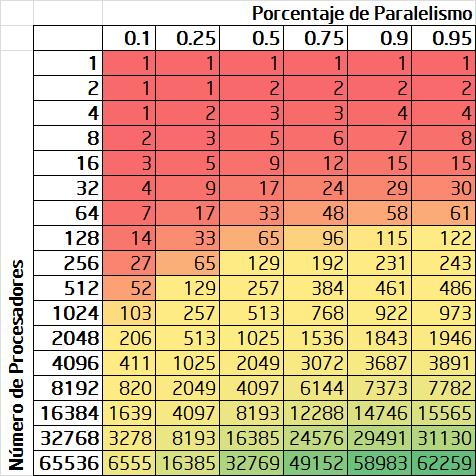
\includegraphics[width=7cm]{gustafson.png}
\label{fig:gustafson}
\end{table}

Similarmente al cuadro anterior, podemos deducir de la Tabla \ref{fig:gustafson} que en el caso de un programa con sólo $ 10\% $ de paralelismo, al incrementar los recursos $ 64x $ sólo podemos incrementar el tamaño del problema $ 7x $. En el otro extremo, nos estima un incremento de $ 61x $ en el caso de tener $ 95\% $ de paralelismo.

\subsubsection{Métrica de {\it Karp-Flatt}}

Esta métrica es utilizada para medir el grado de paralelismo de una aplicación \cite{karp-flatt}. Su valor nos permite rápidamente dimensionar la mejora posible al aplicar un alto nivel de paralelismo.

\bigskip

Dado un cómputo paralelo con una mejora de rendimiento $ \psi $ en $ P $
procesadores, donde $ P > 1 $. La fracción serial {\it Karp-Flatt} representada con $ e $ y calculada según la Ecuación \ref{eq:karp-flatt} es determinada experimentalmente, mientras menor sea $ e $ mayor se supone el nivel de paralelismo posible.

\begin{eqnarray}
\label{eq:karp-flatt}
 e = \frac{\frac{1}{\psi} - \frac{1}{p}}{1 - \frac{1}{p}} 
\end{eqnarray}

Para un problema de tamaño fijo, la eficiencia típicamente disminuye cuando el número de procesadores aumenta. Se puede entonces determinar si esta disminución es debida a un paralelismo limitado, a un algoritmo no optimizado o un problema de arquitectura del sistema.

\subsection{Métricas}

Algunos ejemplos de medida de rendimiento son:

\begin{enumerate}
\item El ancho de banda y la latencia mínima de un canal de comunicación,
  una jerarquía de memorias o de la unidad de almacenamiento.
\item La cantidad de instrucciones, operaciones, datos o trabajo procesado
  por cierta unidad de tiempo.
\item El rendimiento asociado al costo del equipamiento, incluyendo mantenimiento
 periódico, personal dedicado y gastos propios del uso cotidiano.
\item El rendimiento por unidad de energía consumida (electricidad).

\end{enumerate}

Un método de medición de rendimiento indirecto consiste en medir el uso de
los recursos del sistema mientras se ejercita el mismo con un trabajo dado.
Por ejemplo: el nivel de carga de trabajo en el sistema, la cantidad de operaciones realizadas por el
sistema operativo o la unidad de procesamiento, la utilización de memoria o
archivos temporales e incluso el ancho de banda de red utilizado durante la comunicación.

\subsection{Técnicas de Análisis}

El procedimiento de mejora general usualmente consiste en ciclos iterativos de medir, localizar, optimizar y
comparar (Figura \ref{fig:cycle}). Es muy importante mantener la disciplina en realizar un cambio a la
vez ya que esto asegura resultados reproducibles y convergentes, sin efectos no deseados.

\begin{figure}[H]
\begin{center}
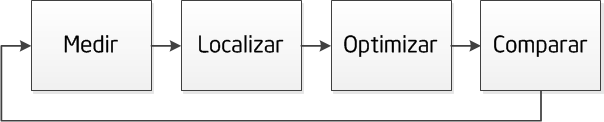
\includegraphics[width=10cm]{cycle.png}
\caption{Optimización Iterativa}
\label{fig:cycle}
\end{center}
\end{figure}

A la hora de tomar decisiones, éstas deben estar basadas en datos concretos, ya que en caso contrario se podría estar trabajando sin llegar a obtener un rédito adecuado.

\bigskip

En el caso de tener problemas de desviación en los resultados medidos, es aconsejable obtener un gran número de muestras y utilizar un valor promedio para asegurarse de evitar errores de medición tanto como sea posible. También es preferible aumentar el tamaño del problema a resolver, o la definición de los resultados para ejercitar por más tiempo y tener así un resultado más estable.
Suponiendo una distribución normal de resultados, se suelen controlar que haya menos de 3 $ \sigma $ de diferencia. Se busca que la mayoría de los resultados queden cerca de su promedio, como muestra la Figura \ref{fig:deviation}.

\begin{figure}[H]
\centering
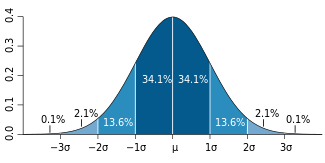
\includegraphics[width=8cm]{deviation.png}
\caption{Desviación de valores en una distribución normal [Wikipedia]}
\label{fig:deviation}
\end{figure}

Los resultados deben también ser correctamente guardados para evitar
problemas de datos. Si la configuración del sistema es dinámica entonces la
reproducción de resultados es no trivial. En el caso de no tener una
configuración de sistema estable en el tiempo, es recomendable siempre
ejecutar una versión optimizada contra una versión de referencia en un mismo
sistema de cómputo.

\bigskip

Para comparar es recomendable utilizar la media geométrica según la Ecuación \ref{eq:geomean} en lugar de la aritmética \cite{how-not-to-lie}, ya que permite dimensionar la tendencia central de un valor típico en un conjunto de números. Esto permite reducir el impacto de ruido introducido por una ejecución problemática.

\begin{equation}
\label{eq:geomean}
G = \sqrt[n]{x_{1} \ldots x_{n}}
\end{equation}

La raíz n-ésima de un número (para un $ n $ posiblemente muy grande), es una operación ineficiente ya que se implementa con métodos numéricos de aproximación siguiendo el método de {\it Newton} \cite{numerical-analysis}. En cambio se suele tomar el anti-logaritmo del promedio de los logaritmos de los valores siguiendo la ecuación \ref{eq:geomean-log}.

\begin{equation}
\label{eq:geomean-log}
G = 10 ^{( log _{10} (x_{1}) + \ldots + log _{10} (x_{n}) ) / n}
\end{equation}

\section{Herramientas}

Actualmente existen numerosas y diversas herramientas para el análisis de rendimiento \cite{gregg}. Estas funcionan a diferentes niveles de abstracción: desde contadores de eventos a nivel de {\it hardware}, pasando por monitores de recursos dentro del núcleo del sistema operativo, instrumentación de código, y hasta la simple utilización del tiempo de ejecución de una aplicación o la comparación contra un trabajo similar de referencia. Para poder analizar del rendimiento un desarrollador aplica las herramientas listadas en la Tabla \ref{table:tools}.

\begin{table}[H]
    \caption{Herramientas de Soporte para Optimización}
    \centering
    \begin{tabular}{|l|l|}\hline
      {\bf Ejemplo} & {\bf Descripción} \\ \hline
      Software {\tt gprof} & Muestra información de perfil de llamadas a funciones \\ \hline
      Hardware {\tt perf} & Muestra información de perfil de sistema \\ \hline
      {\it STREAM} & Benchmark de jerarquía de memoria \\ \hline
      HPL & Benchmark de capacidad de cómputo \\ \hline
      IMB Ping Pong & Benchmark de latencia y ancho de banda de red \\ \hline
      HPCC & Paquete de benchmarks \\ \hline
    \end{tabular}
    \label{table:tools}
\end{table}

Las pruebas de rendimiento como STREAM, HPL, IMB Ping Pong y HPCC permiten conocer el estado del sistema y los límites de rendimiento en la práctica.
Los perfiles de ejecución de aplicaciones y sistema permiten conocer como se utilizan los recursos del sistema para llevar a cabo las instrucciones de cada programa.

\subsection{Pruebas de Rendimiento}

Para medir el rendimiento se utilizan pruebas de referencia ({\em benchmarks}); éstas pueden ser aplicaciones sintéticas construidas específicamente, o bien aplicaciones del mundo real computando un problema prefijado. Al tener valores de referencia se pueden caracterizar los sistemas de modo de predecir el rendimiento de una aplicación.
Los valores a los que se llegan con un {\it benchmark} suelen ser más prácticos y
comparables que los teóricos de acuerdo a condiciones ideales de uso de recursos.
También es posible garantizar que el sistema sigue en un mismo estado con el correr
del tiempo y después de cambios de configuraciones en {\it hardware} o {\it software}.

\bigskip

Las características deseables en un {\it benchmark} son portabilidad, simplicidad, estabilidad y
reproducción de resultados. Esto permite que sean utilizadas para realizar
mediciones cuantitativas y así realizar comparaciones de optimizaciones o
entre sistemas de cómputo diferentes. También se pide que el tiempo de
ejecución sea razonable y que el tamaño del problema sea ajustable para
poder mantener su utilidad con el paso del tiempo y el avance de las
tecnologías.

\bigskip

A continuación se introducen algunas de las más utilizadas para cómputo
de altas prestaciones (listadas en la tabla \ref{table:benchmark-list}),
y posteriormente algunos detalles específicos e instancias
de sus datos de salida para ser utilizados a manera de ejemplo.

\begin{table}[H]
    \caption{Benchmarks}
    \centering
    \begin{tabular}{|l|l|l|}\hline
      {\bf Benchmark} & {\bf Componente} & {\bf Descripción} \\ \hline
      STREAM & Memoria & Ancho de banda sostenido \\ \hline
      Linpack & Procesador & Operaciones de punto flotante \\ \hline
      IMB Ping Pong & Red & Latencia/Ancho de banda de red \\ \hline
      HPCC & Sistema & Múltiples componentes \\ \hline
        \end{tabular}
  \label{table:benchmark-list}
\end{table}

\bigskip

Los {\it benchmarks} pueden ser utilizados para diferentes propósitos. Primero,
los valores reportados son usados como referencia para contrastar rendimiento.
Segundo, su desviación demuestra que algo ha cambiado en el sistema (por lo tanto
su no desviación indica que el sistema sigue saludable). Por último,
un {\it benchmark} sintético implementando el cómputo que uno quiere realizar
muestra el rendimiento máximo posible a obtener en la práctica.

\subsubsection{STREAM}

STREAM \cite{stream} es un {\it benchmark} sintético que mide el ancho de banda de memoria sostenido en MB/s y el rendimiento de computación relativa de algunos vectores simples de cálculo. Se utiliza para dimensionar el ancho de banda de acceso de escritura o lectura a la jerarquía de memoria principal del sistema bajo análisis. Dentro de una misma ejecución de este {\it benchmark} se ejercitan diferentes operaciones en memoria, listadas en la tabla \ref{table:stream}.

\begin{table}[H]
\caption{Operaciones del Benchmark STREAM}
  \centering
    \begin{tabular}{|l|l|l|}\hline
      {\bf Función} & {\bf Operación} & {\bf Descripción} \\ \hline
      {\tt copy} & $ \forall i $ $ b_{i} = a_{i} $ & Copia simple \\ \hline
      {\tt scale} & $ \forall i $ $ b_{i} = c \times a_{i} $ & Multiplicación escalar \\ \hline
      {\tt add} & $ \forall i $ $ c_{i} = b_{i} + a_{i} $ & Suma directa \\ \hline
      {\tt triad} & $ \forall i $ $ c_{i} = b_{i} + c \times a_{i} $ & Suma y multiplicación escalar \\ \hline
    \end{tabular} 
 \label{table:stream}
\end{table}

La salida en pantalla muestra entonces los diferentes tiempos conseguidos y la cantidad de información transferida por unidad de tiempo.
Como último paso, el programa valida también la solución computada.

{\small
\begin{verbatim}
  STREAM version $Revision: 1.2 $
  -------------------------------------------------------------
  This system uses 8 bytes per DOUBLE PRECISION word.
  -------------------------------------------------------------
  Array size = 10000000, Offset = 0
  Total memory required = 228.9 MB.
  Each test is run 10 times, but only the *best* time is used.
  -------------------------------------------------------------
  Function     Rate (MB/s)   Avg time     Min time     Max time
  Copy:        4764.1905       0.0337       0.0336       0.0340
  Scale:       4760.2029       0.0338       0.0336       0.0340
  Add:         4993.8631       0.0488       0.0481       0.0503
  Triad:       5051.5778       0.0488       0.0475       0.0500
  -------------------------------------------------------------
  Solution Validates
\end{verbatim}
}

\subsubsection{Linpack}

Linpack \cite{linpack} es un conjunto de subrutinas {\it FORTRAN} que resuelven
problemas de álgebra lineal como ecuaciones lineales y multiplicación de
matrices. High Performance Linpack (HPL) \cite{hpl} es una versión portable del {\it benchmark} que incluye
el paquete Linpack pero modificado para sistemas de memoria distribuida.

\bigskip

Este {\it benchmark} es utilizado mundialmente para la comparación de la
velocidad de las supercomputadoras en el ranking TOP500. 
Un gráfico del TOP500 de los últimos años (Figura \ref{fig:top500}) demuestra claramente la
tendencia en crecimiento de rendimiento; también la relación entre el primero,
el último y la suma de todos los sistemas en la lista.

\begin{figure}[H]
\centering
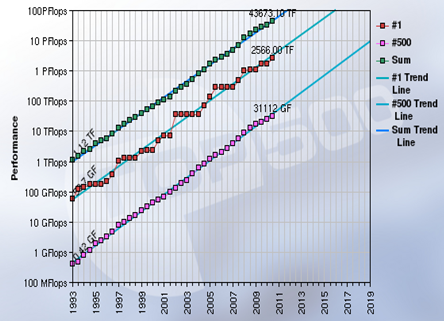
\includegraphics[width=12cm]{top500.png}
\caption{Rendimiento Agregado del Top500 [Top500])}
\label{fig:top500}
\end{figure}

Este {\it benchmark} requiere conocimiento avanzado para una correcta configuración,
por ejemplo el tamaño de bloque que se va a utilizar para la distribución de trabajo
debe estar directamente relacionado con el tamaño del {\it cache} de memoria del procesador.

\bigskip

La salida en pantalla resume entonces los datos de entrada y los resultados conseguidos.
Como último paso el programa valida que los resultados sean correctos.

{\small
\begin{verbatim}
=================================================================
HPLinpack 2.0 - High-Performance Linpack benchmark - Sep 10, 2008
Written by A. Petitet and R. Clint Whaley
=================================================================
The following parameter values will be used:
N      :   28888
NB     :     168
PMAP   : Row-major process mapping
P      :       4
Q      :       4
PFACT  :   Right
NBMIN  :       4
NDIV   :       2
RFACT  :   Crout
BCAST  :  1ringM
DEPTH  :       0
SWAP   : Mix (threshold = 64)
L1     : transposed form
U      : transposed form
EQUIL  : yes
ALIGN  : 8 double precision words
------------------------------------------------------------------
- The matrix A is randomly generated for each test.
- The relative machine precision (eps) is taken to be 1.110223e-16
- Computational tests pass if scaled residuals are less than 16.0

Column=000168 Fraction=0.005 Mflops=133122.97
...
Column=025872 Fraction=0.895 Mflops=98107.60
======================================================================
T/V                N   NB   P    Q             Time             Gflops
WR01C2R4       28888  168   4    4           165.83          9.693e+01
----------------------------------------------------------------------
||Ax-b||_oo/(eps*(||A||_oo*||x||_oo+||b||_oo)*N) = 0.0043035 .. PASSED
======================================================================
Finished      1 tests with the following results:
1 tests completed and passed residual checks,
0 tests completed and failed residual checks,
0 tests skipped because of illegal input values.
\end{verbatim}
}

\bigskip

Existe cierta controversia de que no es una buena forma de ejercitar un
sistema de cómputo distribuido ya que no implica uso significativo de la
red, sólo procesamiento intensivo de aritmética de punto flotante
sobre la jerarquía local de memoria.

\subsubsection{Intel MPI Benchmarks}

Es un conjunto de {\it benchmarks} cuyo objetivo es ejercitar las funciones
más importantes del estándar para librerías de paso de mensajes (MPI, por sus siglas en inglés) \cite{mpi-standard}.
El más conocido es el popular ping-pong, el cual ejercita la transmisión de mensajes ida y vuelta entre dos nodos de
cómputo con diferentes tamaños de mensajes. \cite{latency}.

\bigskip

Para obtener el máximo ancho de banda disponible, se ejercita la comunicación a través de mensajes con datos grandes. Para obtener la mínima latencia, se ejercita la comunicación con mensajes vacíos.

{\small
\begin{verbatim}
# Intel (R) MPI Benchmark Suite V3.1, MPI-1 part
# Date                  : Wed Mar  3 10:45:16 2010
# Machine               : x86_64
# System                : Linux
# Release               : 2.6.16.46-0.12-smp
# Version               : #1 SMP Thu May 17 14:00:09 UTC 2007
# MPI Version           : 2.0
# MPI Thread Environment: MPI_THREAD_SINGLE
# Calling sequence was: ../IMB-MPI1 pingpong
# Minimum message length in bytes:   0
# Maximum message length in bytes:   4194304
#
# MPI_Datatype                   :   MPI_BYTE
# MPI_Datatype for reductions    :   MPI_FLOAT
# MPI_Op                         :   MPI_SUM
#
# List of Benchmarks to run: PingPong
#---------------------------------------------------
# Benchmarking PingPong
# #processes = 2
#---------------------------------------------------
#bytes     #repetitions  t[usec]     Mbytes/sec
0              1000           17.13        0.00
1              1000           17.89        0.05
2              1000           17.82        0.11
4              1000           17.95        0.21
...
1048576    40              8993.23    111.19
2097152    20              17919.20  111.61
4194304    10              35766.45  111.84
\end{verbatim}
}

\subsubsection{HPC Challenge}

El {\it benchmark} HPC Challenge \cite{hpcc} (HPCC) está compuesto internamente por un conjunto de
varios núcleos de cómputo: entre ellos STREAM, HPL, Ping Pong, Transformadas de {\it Fourier}
y otros ejercitando la red de comunicación.

\bigskip

Este benchmark muestra diferentes resultados que son representativos
y puestos en consideración de acuerdo al tipo de aplicación en discusión.
La mejor máquina depende de la aplicación específica a ejecutar, ya que algunas
aplicaciones necesitan mejor ancho de banda de memoria, mejor canal de comunicación, o
simplemente la mayor capacidad de cómputo de operaciones flotantes posible.

\bigskip

Una analogía interesante para entender cómo el {\it benchmark} se relaciona con diferentes núcleos de cómputo se muestra en la Figura \ref{fig:locality}. Por ejemplo al tener un problema que utiliza principalmente acceso a memoria local, se puede suponer que un sistema con buenos resultados de STREAM va ser útil.

\begin{figure}[H]
\begin{center}
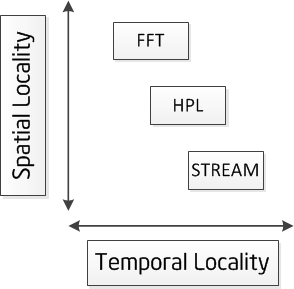
\includegraphics[width=10cm]{locality.png}
\caption{Localidad temporal versus espacial en resultados de HPCC}
\label{fig:locality}
\end{center}
\end{figure}

Para una mejor comparación de resultados de HPCC se utilizan diagramas
denominados {\it kiviats}, un ejemplo se muestra en la Figura \ref{fig:kiviat}.
Los resultados están normalizados hacia uno de los sistemas, y se puede identificar mejor rendimiento en FLOPs por poseer mejores DGEMM y HPL en comparación.

\begin{figure}[H]
\begin{center}
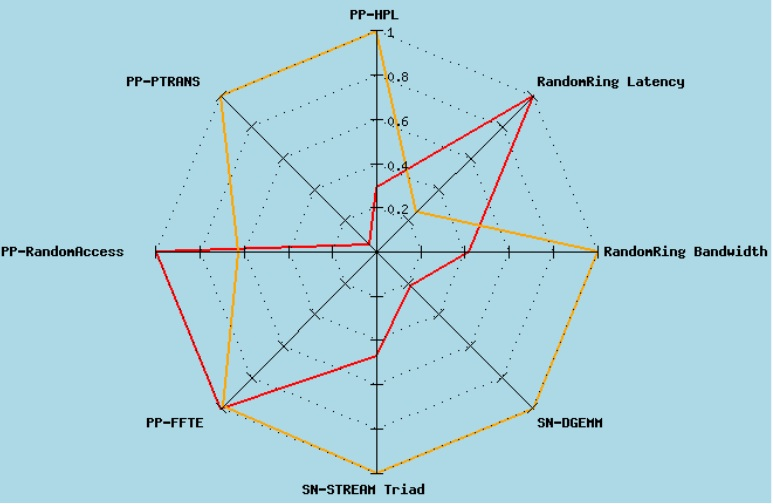
\includegraphics[width=12cm]{kiviat.png}
\caption{Diagrama Kiviat [Top500]}
\label{fig:kiviat}
\end{center}
\end{figure}

Un ejemplo de la salida que se muestra durante la ejecución se muestra a continuación.

{\scriptsize

\begin{verbatim}
This is the DARPA/DOE HPC Challenge Benchmark version 1.2.0 October 2003
Produced by Jack Dongarra and Piotr Luszczek
Innovative Computing Laboratory
University of Tennessee Knoxville and Oak Ridge National Laboratory

Begin of Summary section.
\end{verbatim}

\begin{minipage}[b]{0.5\linewidth}
\begin{verbatim}
VersionMajor=1
VersionMinor=2
LANG=C
Success=1
CommWorldProcs=3
MPI_Wtick=1.000000e-06
HPL_Tflops=0.0674008
HPL_time=26.3165
HPL_eps=1.11022e-16
HPL_N=13856
HPL_NB=64
HPL_nprow=1
HPL_npcol=3
HPL_depth=2
HPL_nbdiv=2
HPL_nbmin=8
HPL_cpfact=C
HPL_crfact=R
HPL_ctop=1
HPL_order=R
dweps=1.110223e-16
sweps=5.960464e-08
HPLMaxProcs=3
HPLMinProcs=3
DGEMM_N=4618
StarDGEMM_Gflops=68.9053
SingleDGEMM_Gflops=70.2692
PTRANS_GBs=0.794254
PTRANS_time=0.479293
PTRANS_residual=0
PTRANS_n=6928
PTRANS_nb=64
PTRANS_nprow=1
PTRANS_npcol=3
MPIRandomAccess_N=134217728
MPIRandomAccess_time=30.4475
MPIRandomAccess_Check=14.0705
MPIRandomAccess_Errors=0
\end{verbatim}
\end{minipage}
\hspace{0.1cm}
\begin{minipage}[b]{0.5\linewidth}
\begin{verbatim}
MPIRandomAccess_ErrorsFraction=0
MPIRandomAccess_ExeUpdates=536870912
MPIRandomAccess_GUPs=0.0176327
MPIRandomAccess_TimeBound=-1
MPIRandomAccess_Algorithm=0
RandomAccess_N=33554432
StarRandomAccess_GUPs=0.0186362
SingleRandomAccess_GUPs=0.0184568
STREAM_VectorSize=21332081
STREAM_Threads=8
StarSTREAM_Copy=4.34705
StarSTREAM_Scale=3.24366
StarSTREAM_Add=3.41196
StarSTREAM_Triad=3.46198
SingleSTREAM_Copy=4.53628
SingleSTREAM_Scale=3.38984
SingleSTREAM_Add=3.59073
SingleSTREAM_Triad=3.65083
FFT_N=8388608
StarFFT_Gflops=2.17339
SingleFFT_Gflops=2.26806
MPIFFT_N=8388608
MPIFFT_Gflops=1.7043
MPIFFT_maxErr=1.77722e-15
MPIFFT_Procs=2
MaxPingPongLatency_usec=5.37932
RandomRingLatency_usec=5.70686
MinPingPongBandwidth_GBytes=0.675574
NaturalRingBandwidth_GBytes=0.531278
RandomRingBandwidth_GBytes=0.529161
MinPingPongLatency_usec=5.24521
AvgPingPongLatency_usec=5.30978
MaxPingPongBandwidth_GBytes=0.682139
AvgPingPongBandwidth_GBytes=0.678212
NaturalRingLatency_usec=5.79357
FFTEnblk=16
FFTEnp=8
FFTEl2size=1048576
\end{verbatim}
\end{minipage}

\begin{verbatim}
End of Summary section.
End of HPC Challenge tests.
\end{verbatim}
}

\subsection{Herramientas}

Se recomienda un proceso de aplicación gradual empezando por herramientas generales de alto nivel que analizan la aplicación como un todo; terminando con herramientas de bajo nivel que proveen detalles complejos de granularidad más fina en partes específicas del código. Esto permite ir analizando el rendimiento sin tener que enfrentar la dificultad de un análisis complejo y extensivo desde un principio. Una lista de las herramientas más conocidas se muestra en la Tabla \ref{table:tooling}.

\begin{table}[H]
\caption{Aplicación Gradual de Herramientas}
\begin{tabular}{|l|l|} \hline
{\bf Característica} & {\bf Herramientas} \\ \hline
Capacidad del sistema & Benchmark HPCC \\ \hline
Medición de ejecución & {\tt time}, {\tt gettimeofday()}, {\tt MPI\_WTIME()} \\ \hline
Perfil de ejecución & profilers: {\tt gprof, perf} \\ \hline
Comportamiento de la aplicación & profilers: {\tt gprof, perf} \\ \hline
Comportamiento de librerías & profilers: valgrind, MPI vampir. \\ \hline
Comportamiento del sistema & profilers: oprofile, perf \\ \hline
Vectorización & compilador: gcc \\ \hline
Contadores en {\it hardware} & oprofile, PAPI, perf \\ \hline
\end{tabular}
\label{table:tooling}
\end{table}

A grandes rasgos el procedimiento es el siguiente:

\begin{enumerate}

\item Se establece una línea de comparación al ejecutar una prueba de rendimiento del sistema, {\it HPCC} brinda un conjunto de métricas muy completo. 

\item Se utilizan herramientas para medir el tiempo de ejecución de la aplicación sobre diferentes escenarios. time permite una ejecución directa sin modificación de código, {\tt gettimeofday()} requiere modificación de código pero puede ser utilizados con mayor libertad dentro de la aplicación.  
En el caso de estar utilizando la librería MPI {\tt MPI\_WTime()} y la herramienta VAMPIR\footnote{\href{http://www.vampir.eu}{http://www.vampir.eu}} proveen soporte específico para análisis de rendimiento.

\item Se dimensiona el comportamiento de la aplicación mediante un perfil de ejecución y un análisis de cuello de botella utilizando {\tt gprof}. 

\item Se analiza el comportamiento del sistema ejecutando la aplicación mediante {\tt oprofile} \footnote{\href{http://oprofile.sourceforge.net}{http://oprofile.sourceforge.net}} o {\tt perf} \footnote{\href{https://perf.wiki.kernel.org}{https://perf.wiki.kernel.org}}. 

\item Se revisa el reporte del compilador para comprobar que se estén vectorizando los ciclos de cálculo más intensivos.

\item Se analiza el comportamiento de las unidades de cómputo utilizando soporte de {\it hardware} mediante herramientas como {\tt perf}, {\tt oprofile} y {\it Performance Application Programming Interface} (PAPI) \footnote{\href{http://icl.cs.utk.edu/papi}{http://icl.cs.utk.edu/papi}}.

\end{enumerate}

\subsection{Tiempo de Ejecución}

Esta sección revisa como medir el tiempo de ejecución global de una aplicación, incluyendo ejemplos.

\subsubsection{Tiempo de ejecución global}

Para medir el tiempo de ejecución de un comando en consola se utiliza {\tt time(1)}. Aunque rudimentaria, esta simple herramienta no necesita de instrumentación de código y se encuentra disponible en cualquier distribución {\it GNU/Linux}.
El intérprete de comandos tiene su propia versión embebida, sin embargo el del sistema brinda información del uso de otros recursos del sistema, usualmente localizado en {\tt /usr/bin/time}.

\bigskip

\begin{lstlisting}
$ /usr/bin/time -v ./program
1
        Command being timed: "./program"
        User time (seconds): 0.61
        System time (seconds): 0.00
        Percent of CPU this job got: 99%
        Elapsed (wall clock) time (h:mm:ss or m:ss): 0:00.62
        Average shared text size (kbytes): 0
        Average unshared data size (kbytes): 0
        Average stack size (kbytes): 0
        Average total size (kbytes): 0
        Maximum resident set size (kbytes): 4560
        Average resident set size (kbytes): 0
        Major (requiring I/O) page faults: 0
        Minor (reclaiming a frame) page faults: 668
        Voluntary context switches: 6
        Involuntary context switches: 2
        Swaps: 0
        File system inputs: 0
        File system outputs: 0
        Socket messages sent: 0
        Socket messages received: 0
        Signals delivered: 0
        Page size (bytes): 4096
        Exit status: 0
\end{lstlisting}

\subsubsection{Reloj del sistema}

La librería de sistema permite acceder a llamadas al sistema operativo para obtener datos precisos del paso del tiempo.
Las más utilizadas son {\tt gettimeofday(3)} y {\tt clock(3)}, aunque éste último se comporta de manera especial al utilizar multi-threading ya que suma el tiempo ejecutado en cada core.

\bigskip

El siguiente código ejemplifica como obtener un número de segundos en una representación de punto flotante de doble precisión, permitiendo una granularidad de medición adecuada.

\begin{lstlisting}
double wtime(void)
{
  double sec;
  struct timeval tv;
  
  gettimeofday(&tv, NULL);
  sec = tv.tv_sec + tv.tv_usec/1000000.0;
  return sec;
}
\end{lstlisting}

\subsection{Perfil de Ejecución Funcional}

Estas herramientas denominadas {\it profilers} extraen el perfil dinámico de una aplicación en tiempo de ejecución. 
Se instrumenta la aplicación con una opción específica que incluye información de uso de las diferentes partes del programa y los recursos del sistema como por ejemplo procesador y memoria.

\bigskip

La aplicación debe ejecutarse con un conjunto de datos prefijado. El conjunto de
datos debe ser representativo y debe también ejercitar la aplicación por
una cantidad de tiempo suficiente como para intensificar el uso de los
recursos. Los datos del perfil de una ejecución son luego obtenidos en la
forma de un archivo de datos, luego se procede a procesar los datos acumulados
con un analizador respectivo.

\bigskip

Provee un perfil plano que consiste en una simple lista de las funciones
ejecutadas ordenadas por la cantidad acumulada de tiempo utilizado.
También provee el gráfico de llamadas anidadas, que muestra el tiempo
utilizado por cada función en llamadas sucesivas. Las funciones recursivas
son manejadas de manera especial ya que imposibilitan el armado de relaciones
de dependencias.

\subsubsection{Ejemplo: {\tt gprof}}

El perfil de ejecución de {\tt gprof} muestra el tiempo individual y el tiempo acumulado en segundos de cada línea de código de la aplicación. Los binarios deben ser compilados con información extra de depuración, en el caso de {\tt gcc}, las opciones necesarias son {\tt -g -pg}. Si {\tt -g} no se encuentra presente entonces no se provee el reporte detallado por línea de ejecución. Esto permite identificar donde se está consumiendo tiempo durante la ejecución.
La herramienta también muestra un cuadro de las llamadas entre funciones realizadas por el programa.
Esto permite visualizar el esquema de dependencias durante la ejecución.

\bigskip

A continuación se muestra como realizar la compilación incluyendo información de depuración específica, además de un caso concreto contra una aplicación simulando el juego de la vida \cite{conway}.

\begin{lstlisting} 
$ gcc -g -pg program.c -o program
$ ./program
$ gprof program
...
\end{lstlisting}

\begin{lstlisting} 
Flat profile:
Each sample counts as 0.01 seconds.
% cumulative self self total
time seconds seconds calls us/call us/call name
37.50 0.15 0.15 48000 3.12 3.12 Life::neighbor_count(int, int)
...
\end{lstlisting}

\begin{lstlisting} 
Call graph
granularity: each sample hit covers 4 byte(s) for 2.50% of 0.40 seconds
index % time    self  children    called     name
      0.02 0.15 12/12 main [2]
[1] 42.5 0.02 0.15 12 Life::update(void) [1]
      0.15 0.00 48000/48000 Life::neighbor_count(int, int) [4]
--
          0.00    0.17       1/1           _start [3]
[2]     42.5    0.00    0.17       1         main [2]
          0.02    0.15      12/12          Life::update(void) [1]
          0.00    0.00      12/12          Life::print(void) [13]
          0.00    0.00      12/12          to_continue(void) [14]
          0.00    0.00       1/1           instructions(void) [16]
          0.00    0.00       1/1           Life::initialize(void) [15]
--
\end{lstlisting}

\subsection{Perfil de Ejecución Asistido por {\it Hardware}}

Un {\it profiler} puede utilizar el {\it hardware} para analizar el uso de los recursos disponibles a nivel de núcleo del
sistema operativo. Actúa de forma transparente a nivel global. Utiliza
contadores de {\it hardware} del CPU y utiliza interrupciones de un temporizador
cuando no logra detectar soporte específico en {\it hardware}. Aunque tiene un costo adicional inherente, la sobrecarga es mínima.

\bigskip

Para obtener un perfil de ejecución representativo, usualmente se recomienda detener toda aplicación o servicio no relevante en el sistema. La herramienta de por si no requiere acceder al código fuente de la aplicación, pero si esta disponible el código correspondiente se muestra anotado con contadores si hay símbolos de depuración en el binario.

\bigskip

Los registros de {\it hardware} implementando contadores más utilizados son los
siguientes:

\begin{enumerate}
\item Cantidad total de ciclos de procesador
\item Cantidad total de instrucciones ejecutadas
\item Cantidad de ciclos detenidos por espera de acceso a memoria
\item Cantidad de instrucciones de punto flotante
\item Cantidad de fallos de cache de nivel uno (L1)
\item Cantidad de instrucciones de carga y descarga
\end{enumerate}

En núcleos más viejos que la versión 2.6, en lugar de {\tt oprofile} se recomienda utilizar {\tt perf}. Al estar implementados a nivel de núcleo, éstos evitan las llamadas al sistema y tienen una sobrecarga de un orden de magnitud menor que los {\it profilers} a nivel de aplicación. Las herramientas propietarias suelen tener acceso a contadores más específicos e
incluso programables para funciones determinadas de medición.

\subsubsection{Ejemplo: {\tt perf}}

A continuación se demuestra la información provista por {\tt perf} en sus diferentes modos de ejecución: estadísticas de contadores, perfil de sistema y por último perfil de aplicación.

\begin{lstlisting}
$ perf stat -B program

Performance counter stats for 'program':

           5,099 cache-misses  0.005 M/sec (scaled from 66.58%)
         235,384 cache-references 0.246 M/sec (scaled from 66.56%)
       9,281,660 branch-misses 3.858 %     (scaled from 33.50%)
     240,609,766 branches 251.559 M/sec (scaled from 33.66%)
   1,403,561,257 instructions  0.679 IPC   (scaled from 50.23%)
   2,066,201,729 cycles 2160.227 M/sec (scaled from 66.67%)
             217 page-faults 0.000 M/sec
               3 CPU-migrations 0.000 M/sec
              83 context-switches 0.000 M/sec
      956.474238 task-clock-msecs 0.999 CPUs

      0.957617512  seconds time elapsed
\end{lstlisting}

\begin{lstlisting}
$ perf record ./mm
$ perf report
# Events: 1K cycles
# Overhead Command Shared Object Symbol
28.15% main mm [.] 0xd10b45
4.45% swapper  [kernel.kallsyms] [k] mwait_idle_with_hints
4.26% swapper  [kernel.kallsyms] [k] read_hpet
...
\end{lstlisting}

\begin{lstlisting}
 Percent |   Source code & Disassembly of program
         :   Disassembly of section .text:
         :   08048484 <main>:
         :   #include <string.h>
         :   #include <unistd.h>
         :   #include <sys/time.h>
         :
         :   int main(int argc, char **argv)
         :   {
0.00:    8048484:       55                      push   %ebp
0.00:    8048485:       89 e5                   mov    %esp,%ebp
...
0.00:    8048530:       eb 0b                   jmp 804853d <main+0xb9>
         :                           count++;
14.22:    8048532:       8b 44 24 2c             mov    0x2c(%esp),%eax
0.00:    8048536:       83 c0 01                add    $0x1,%eax
14.78:    8048539:       89 44 24 2c             mov    %eax,0x2c(%esp)
         :           memcpy(&tv_end, &tv_now, sizeof(tv_now));
         :           tv_end.tv_sec += strtol(argv[1], NULL, 10);
         :           while (tv_now.tv_sec < tv_end.tv_sec ||
         :                  tv_now.tv_usec < tv_end.tv_usec) {
         :                   count = 0;
         :                   while (count < 100000000UL)
14.78:    804853d:       8b 44 24 2c             mov    0x2c(%esp),%eax
56.23:    8048541:       3d ff e0 f5 05          cmp    $0x5f5e0ff,%eax
0.00:    8048546:       76 ea                   jbe 8048532 <main+0xae>
...
\end{lstlisting}

Este punto de análisis requiere conocimiento avanzado de como funciona el CPU utilizado, su acceso a memoria y los costos de las diferentes instrucciones soportadas. Una fuente de consulta debe incluir conceptos generales de arquitectura de procesadores \cite{hennessy} e información de los fabricantes \cite{intel-optimization}.

\subsection{Reporte de Vectorización}

Una herramienta de bajo nivel para analizar rendimiento es el mismo compilador
que debería estar vectorizando los ciclos de cómputo intensivo. Esto es muy
útil para detectar si los cuellos de botella ya se encuentran optimizados o no.

\bigskip

Por ejemplo, GCC provee opciones específicas que deben ser provistas para mostrar el reporte.

\begin{lstlisting}
$ gcc -c -O3 -ftree-vectorizer-verbose=1 ex.c
ex.c:7: note: LOOP VECTORIZED.
ex.c:3: note: vectorized 1 loops in function.
$ gcc -c -O3 -ftree-vectorizer-verbose=2 ex.c
ex.c:10: note: not vectorized: complicated access pattern.
ex.c:10: note: not vectorized: complicated access pattern.
ex.c:7: note: LOOP VECTORIZED.
ex.c:3: note: vectorized 1 loops in function.
$ gcc -c -O3 -fdump-tree-vect-details ex.c
...
\end{lstlisting}

En el caso de existir código recursivo, podemos comprobar que no suele estar soportado por los compiladores actuales.

\begin{lstlisting}
$ gcc -Wall -Wextra -O3 -ftree-vectorizer-verbose=4 -g queen.c
queen.c:22: note: vectorized 0 loops in function.
queen.c:35: note: vectorized 0 loops in function.
\end{lstlisting}

\chapter{Descripción del Problema}

Este capítulo introduce el problema a resolver.

\section{Análisis de Rendimiento}

Este trabajo entonces trata de simplificar la tarea de análisis de rendimiento. Aunque es una tarea difícil de sistematizar y que muchas veces depende fuertemente de la aplicación bajo análisis, se propone un procedimiento general para ciertas aplicaciones.

\chapter{Propuesta de Solución}

Este capítulo muestra la propuesta de solución, incluyendo el diseño de la misma a diferentes niveles, un ejemplo de su reporte de salida y realizando casos de aplicación con aplicaciones del mundo real.

\section{Procedimiento}

La Figura \ref{fig:procedure} muestra a grandes rasgos las etapas del proceso.
Primero se establece una línea base de rendimiento del sistema utilizando pruebas conocidas.
Luego se procede a trabajar en etapas iterativas asegurando en cada paso la estabilidad de los resultados, una correcta utilización de recursos y utilizando un perfil de ejecución. Luego de optimizar y comprobar la mejora, se vuelve a empezar el ciclo.

\begin{figure}[H]
\label{fig:procedure}
\centering
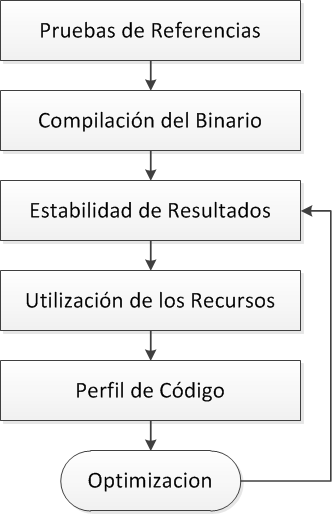
\includegraphics[width=5cm]{procedure.png}
\caption{Procedimiento de Análisis}
\end{figure}

\section{Paso a Paso}

A continuación se muestran los pasos a realizar, junto con preguntas que guían el análisis de rendimiento de una aplicación.

\subsection{Pruebas de Referencia}

\begin{enumerate}
\item Ejecutar pruebas de rendimiento sobre el sistema a utilizar para poder entender sus capacidades máximas en contraste con las teóricas.

\begin{lstlisting}
$ sudo apt-get install hpcc
$ mpirun -n `grep -c proc /proc/cpuinfo` ./hpcc
$ cat hpccoutf.txt
\end{lstlisting}

\begin{enumerate}
\item ¿Los resultados reflejan las capacidades esperadas del sistema?
\item ¿Los FLOPS se aproximan al rendimiento de un sistema similar?
\item ¿El rendimiento es $ CORES \times CLOCK \times FLOPS/CYCLE $ ?
\item ¿La latencia y ancho de banda de la memoria es la esperada?
\end{enumerate}

\item Comprobar variación de resultados para conocer la estabilidad de los mismos. La desviación estándar debe ser menor a 3 sigmas. Establecer cual es el promedio geométrico  a usar como referencia para comparaciones futuras.

\begin{lstlisting}
$ for i in `seq 1 32`; do /usr/bin/time -v ./app >> time.csv; done
\end{lstlisting}

\begin{enumerate}
\item ¿Son los resultados estables?
\item ¿La desviación estándar es menor que 3?
\item ¿Cuál es el promedio geométrico para comparaciones futuras?
\item ¿ Es necesario incrementar el problema para mejorar la desviación?
\item ¿ Es posible reducir el tiempo sin afectar la desviación?
\end{enumerate}

\item Escalar el problema para dimensionar la cantidad de trabajo según el tamaño del problema.

\begin{lstlisting}
$ for size in `seq 1024 1024 10240`; do /usr/bin/time -v ./app $size >> size.log; done
\end{lstlisting}

\begin{enumerate}
\item ¿Cuál es la relación entre el tiempo de las diferentes ejecuciones?
\item ¿Es la relación lineal o constante?
\end{enumerate}

\item Escalar cómputo para luego calcular límite de mejoras con {\it Amdalah} y {\it Gustafson}.

\begin{lstlisting}
$ for threads in `grep -c proc /proc/cpuinfo | xargs seq 1`; do OMP_NUM_THREADS=$threads ./app >> threads.log; done
\end{lstlisting}

\begin{enumerate}
\item ¿Cuál es la relación entre el tiempo de las diferentes ejecuciones?
\item ¿Es la relación lineal o constante?
\item ¿Qué porcentaje de la aplicación se estima paralelo?
\item ¿Cual es la mejora máxima posible?
\end{enumerate}

\item Generar el perfil de llamadas a funciones dentro de la aplicación para revisar el diseño de la misma y los posibles cuellos de botella a resolver.

\begin{lstlisting}
$ gcc -g -pg app.c -o app
$ ./app
\end{lstlisting}

\begin{lstlisting}
$ gprof --flat-profile --graph --annotated-source app
...
\end{lstlisting}

\begin{enumerate}
\item ¿Cómo esta diseñada la aplicación?
\item ¿Que dependencias en librerías externas tiene?
\item ¿Implementa algún núcleo de cómputo conocido encuadrado dentro de librerías optimizadas como BLAS?
\item ¿En que archivos, funciones y líneas se concentra la mayor cantidad de tiempo de cómputo?
\end{enumerate}

\item Utilizar el profiler a nivel de sistema

\begin{lstlisting}
$ prof stat ./app
$ prof record ./app
$ prof report
\end{lstlisting}

\begin{enumerate}
\item ¿Cómo se comporta el sistema durante la ejecución de la aplicación?
\item ¿Son las métricas de contadores de {\it hardware} las esperadas?
\item ¿Es la aplicación la gran concentradora de los recursos disponibles?
\item ¿Qué instrucciones de {\it hardware} son las utilizadas en el cuello de botella?
\end{enumerate}

\item Comprobar vectorizaciones

\begin{lstlisting}
$ gcc -Wall -Wextra -O3 --report-loop
\end{lstlisting}

\begin{enumerate}
\item ¿Hay ciclos que no pueden ser automáticamente vectorizados?
\end{enumerate}

\end{enumerate}

\section{Infraestructura}

El procedimiento anterior se implementó como una infrastructura automática de generacion de reportes de rendimiento denominada 
{\tt hotspot}. \footnote{El proyecto {\tt hotspot} está disponible en \href{https://github.com/moreandres/hotspot}{https://github.com/moreandres/hotspot}}.
{\it Latex} se utiliza para la generación del reporte final.
Se depende de utilidades como GCC, GNU Make, prof, gprof, pidstat para obtener la información relevante.

\bigskip

Las limitaciones {\it a-priori} que posee la infrastructura son en materia de portabilidad y aplicación. Por el lado de la portabilidad, solo se soportan sistemas GNU/Linux recientes, siendo necesarias un conjunto de utilidades de soporte específicas. Por el lado de la aplicación, solo se soportan programan utilizando tecnología OpenMP multi-hilo.

\section{Teoría de Operación}

Esta sección detalla el funcionamiento de la infraestructura relacionando los componentes.

\bigskip

La herramienta de linea de comando toma como parámetro principal el binario de la aplicación a analizar. Asume por defecto que la aplicación esta construida utilizando Makefile de la forma usual, ya que para algunos pasos de análisis se necesita recompilar la aplicación con información extra de depuración.
En el caso de que no sea así, el archivo de configuración permite la definición de tareas como configuración, compilacion y ejecución del programa.

Otros parámetros necesarios son los datos del rango de tamaños de problema a utilizar, asumidos como {\tt seq(1)}.

\begin{lstlisting}[language=bash, caption={ayuda hotspot}, label={lst:hotspot-help}]
$ hotspot --help
usage: hotspot [-h] [-v] [--config CONFIG] [--debug]

Generate performance report for OpenMP programs.

optional arguments:
  -h, --help            show this help message and exit
  -v, --version         show program's version number and exit
  --config CONFIG, -c CONFIG
                        path to configuration
  --debug, -d           enable verbose logging

Check https://github.com/moreandres/hotspot for details.
$ hotspot
\end{lstlisting}

\bigskip

\begin{lstlisting}[language=bash, caption={configuración hotspot}, label={lst:hotspot-config}]
# hotspot configuration file

[hotspot]

# python format method is used to pass parameters

# range is a seq-like definition for problem size
range=1024,2048,256

# cflags are the compiler flags to use when building
cflags=-O3 -Wall -Wextra

# build is the command used to build the program
build=CFLAGS='{0}' make

# clean is the cleanup command to execute
clean=make clean

# run is the program execution command
run=OMP_NUM_THREADS={0} N={1} ./{2}

# count is the number of runs to check workload stabilization
count=16
\end{lstlisting}


\bigskip

Se utiliza un directorio escondido dentro de la carpeta que contiene la aplicación y se guardan en sub-directorios por fecha y hora las diferentes ejecuciones. Esta información es luego usada para comparación histórica de resultados.

\bigskip

Inicialmente se ejecuta la aplicación múltiples veces para validar que los resultados poseen una desviación saludable. Se resume esta información con un histograma y se hace una aproximación a una distribución de resultados normales como comparación.
Se toma como referencia la media geométrica de los resultados.
La primer ejecución se descarta.

\bigskip

Se ejercita la aplicación dentro del rango de tamaño de problema, por cada punto en el rango se ejecuta múltiples veces para promediar. Se grafican los resultados en un gráfico, posiblemente con escala logarítmica. Se sobrepone una curva ideal suponiendo que el doble de tamaño va a necesitar el doble de tiempo de cómputo.
Se sobrepone también la información más vieja disponible como mecanismo de validación de las optimizaciones.

\bigskip

Se detecta cuantas unidades de procesamiento hay en el sistema. Se utiliza una y luego se itera hasta utilizar todas, se ejecuta múltiples veces la aplicación y se promedia el resultado. Se sobrepone una curva ideal suponiendo {\it speedup} ideal. Se sobrepone también la información más vieja disponible como mecanismo de validación de las optimizaciones.

\bigskip

Utilizando la información anterior, se calcula porcentaje de ejecución en serie y en paralelo. Con esta información se calcula limites según leyes de {\it Amdalah} y {\it Gustafson} para los procesadores disponibles y para un número grande como para visualizar que va a pasar con infinitos procesadores.

\bigskip

Se recompila la aplicación con información extra de depuración y se obtiene información del perfil de ejecución. Se detallan las funciones, las líneas de código y el {assembler} implementado por las mismas.

\bigskip

\begin{figure}[H]
\begin{center}
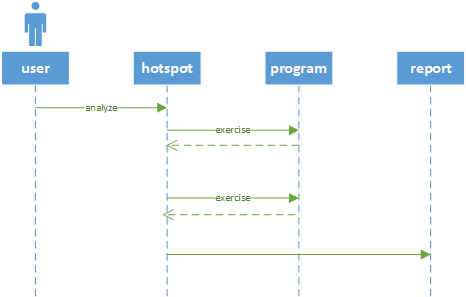
\includegraphics[width=\textwidth]{hotspot-seq.png}
\caption{Diagrama de Secuencia}
\label{fig:hotspot-seq}
\end{center}
\end{figure}

\section{Diseño de Alto Nivel}

El diseño de la infrastructura refleja la interacción manual con el programa a analizar.

\begin{figure}[H]
\begin{center}
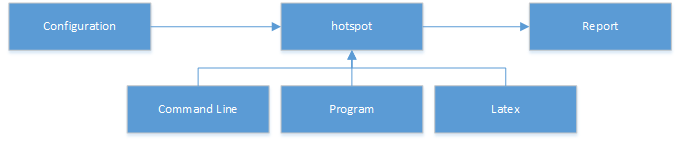
\includegraphics[width=\textwidth]{hotspot-hld.png}
\caption{Diseño de Alto Nivel}
\label{fig:hotspot-hld}
\end{center}
\end{figure}

\begin{enumerate}
\item Configuración, RFC 822
\item componente3
\end{enumerate}

\section{Diseño de Bajo Nivel}

La infrastructura se implementa mediante una jerarquía de clases simple, fácil de extender de ser necesario.

\begin{figure}[H]
\begin{center}
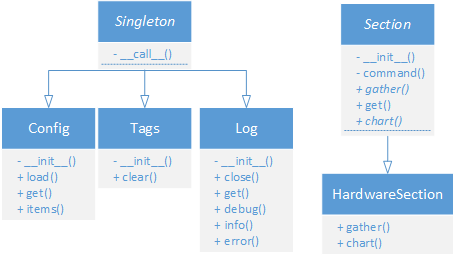
\includegraphics[width=\textwidth]{hotspot-lld.png}
\caption{Diseño de Bajo Nivel}
\label{fig:hotspot-lld}
\end{center}
\end{figure}

\begin{enumerate}
\item Singleton, descripción, responsabilidad
\item Tags, descripción, responsabilidad
\item Log, descripción, responsabilidad
\item Config, descripción, responsabilidad
\item Section, descripción, responsabilidad
\item HardwareSection, descripción, responsabilidad
\item ProgramSection, descripción, responsabilidad
\item SoftwareSection, descripción, responsabilidad
\item SanitySection, descripción, responsabilidad
\item BenchmarkSection, descripción, responsabilidad
\item WorkloadSection, descripción, responsabilidad
\item ScalingSection, descripción, responsabilidad
\item ThreadsSection, descripción, responsabilidad
\item OptimizationSection, descripción, responsabilidad
\item ProfileSection, descripción, responsabilidad
\item ResourcesSection, descripción, responsabilidad
\item AnnotatedSection, descripción, responsabilidad
\item VectorizationSection, descripción, responsabilidad
\item CountersSection, descripción, responsabilidad
\item ConfigSection, descripción, responsabilidad
\end{enumerate}

\section{Reporte Generado}

Secciones dentro del reporte, que datos incluyen y para qué son útiles.

\subsection{Consideraciones Generales}

Las consideraciones generales tenidas en cuenta en todas las secciones fueron las siguientes:

\begin{enumerate}
\item Hipervínculos a archivos con la información pura.
\item Inclusión de una explicación breve de para que sirve la sección y el gráfico.
\item Inclusión de {\it trendlines} y comportamiento ideal.
\item Referencias a material de consulta.
\end{enumerate}

\subsection{Introducción}

Referencia.

\subsection{Estabilidad de Resultados}

Histograma.

\subsection{Escalabilidad}

Tamaño y Procesadores.

\subsection{Mejoras}

Speedup.

\subsection{Profiling}

Funciones más usadas. Cuellos de botella. Líneas de código assembler.

\bigskip

Un ejemplo de salida completo se encuentra adjuntado en el apéndice.

\chapter{Casos de Aplicación}

Este capítulo contiene casos de estudio mostrando los resultados de aplicar la infraestructura desarrollada a aplicaciones de cómputo de alto rendimiento conocidas.

\section{Código de Prueba}

Esta sección incluye los resultados obtenidos al aplicar la infrastructura a núcleos de cómputo de prueba.

\subsection{Matrix}

La multiplicación de matrices es una operación fundamental en múltiples campos de aplicación científica como la resolución de ecuaciones lineales y la representación de grafos y espacios dimensionales. Por ello existe abundante material sobre el tema. Tomando como ejemplo una implementación utilizando OpenMP \footnote{\href{http://blog.speedgocomputing.com/2010/08/parallelizing-matrix-multiplication.html}{http://blog.speedgocomputing.com/2010/08/parallelizing-matrix-multiplication.html}.}

\bigskip

El reporte generado en bruto puede consultarse en el apéndice A.

\subsection{Heat2d}

Otro problema interesante es la simulación de transferencia de calor en un plano.
Se utiliza una grilla donde cada celda transfiere calor a sus vecinos en una serie de ciclos finitas simulando el paso del tiempo \footnote{\href{http://www.rblasch.org/studies/cs580/pa5/\#Source+Code-N100AC}{http://www.rblasch.org/studies/cs580/pa5/\#Source+Code-N100AC}.}.

\bigskip

El reporte generado en bruto puede consultarse en el apéndice B.

\subsection{8 Queens}

El dilema trata en el problema de posicionar en un tablero de ajedrez ocho
reinas sin que alguna amenace a las demás. Una reina amenaza a cualquier otra
pieza en el tablero que este en la mismo diagonal, fila o columna.

El problema de encontrar todas las soluciones para un tamaño de tablero dado suele resolverse utilizando recursión \footnote{\href{http://www.stevenpigeon.org/blogs/hbfs/super-reines-openmp.cpp}{http://www.stevenpigeon.org/blogs/hbfs/super-reines-openmp.cpp}.}.

\bigskip

El reporte generado en brute puede consultarse en el apéndice C.

\section{Código del Mundo Real}

\subsection{NEC OpenMP}

Mario Trangoni realizó una paralelizacion del código original.
Es utilizado por estudiantes de ingeniería electrónica para el cálculo de distribución de radiación de una antena.

\href{bla}{https://code.google.com/p/nec2c/}

Partes relevantes del reporte.

\subsection{Espresso}

Biología. Marcela Moré.

Partes relevantes del reporte.

\section{OpenMP Database (Spain)}

\chapter{Conclusiones y Trabajo Futuro}

Este capítulo concluye revisando los objetivos propuestos y posibles líneas de investigación como continuación.

\section{Conclusiones}

Se desarrollo como esta planeado una infrastructura de soporte que permite a un desarrollador especialista en el dominio de un problema obtener rapidamente  información cuantitativa del comportamiento de un programa OpenMP, incluyendo utilización del recurso y cuellos de botella.

\section{Trabajo Futuro}

Las posibilidades de extensión de esta infrastructura son muchas, cada sección del reporte final puede incluir información más detallada o utilizar otras herramientas. En particular la sección de contadores de {\it hardware} solo contiene una lista de contadores generalizada para cualquier arquitectura; si se supone una arquitectura dada se puede proveer información más especifica y por lo tanto más útil.

\bigskip

Otra posibilidad consiste en incorporar soporte para programas basados sobre la libreria de comunicacion MPI. Una vez que los programas son optimizados para ejecutarse eficientemente sobre una arquitectura multicore, el siguiente paso consiste en utilizar varios sistemas multicore al unísono.

\bigskip

Por último, aunque la generación de un documento portable en formate PDF es simple y útil, se puede pensar en utilizar una tecnología que permita la generacion de reportes dinámicos que permitan a los expertos extraer información. Una implementación en HTML5 utilizando tablas filtrables y gráficos configurables puede ser interesante y causar gran impacto.

\bibliography{report}

\appendix

\chapter{Reporte de Ejemplo}

\section{Multiplicación de Matrices}
% \includepdf[frame=true, pages=-, scale=0.8]{sample.pdf}

\section{Propagación de Calor en 2 Dimensiones}
% \includepdf[frame=true, pages=-, scale=0.8]{sample.pdf}

\section{Problema de las 8 Reinas}
% \includepdf[frame=true, pages=-, scale=0.8]{sample.pdf}

\end{document}
